\documentclass[12pt]{article}
\usepackage{graphicx} % Required for inserting images
\usepackage{enumitem}
\usepackage{amsmath}
\usepackage{gvv-book}
\usepackage{gvv}

\title{\textbf{1.4.19}}
\author{\textbf{EE25BTECH11004 - Aditya Appana}}
\date{August 28, 2025}

\begin{document}

\maketitle

\section*{Question}
Find the acute angle between the planes $ \vec{r} \cdot (\hat{i} - 2\hat{j} - 2\hat{k}) = 1$ and  $ \vec{r} \cdot (3\hat{i} - 6\hat{j} + 2\hat{k}) = 0$

\section*{Solution}
Let the normal vectors be 
\begin{align} 
\vec{n_1}=\myvec{1\\-2\\-2} \\
\vec{n_2}=\myvec{3\\-6\\2}
\end{align}

\vspace{1cm}

The formula to calculate the angle between the two planes is
\begin{align}
\theta = \frac{\pi}{2} - \cos^{-1}\brak{\frac{\vec{n_1}^T\vec{n_2}}{|\vec{n_1}||\vec{n_2}|}}
= \sin^{-1}\brak{\frac{\vec{n_1}^T\vec{n_2}}{|\vec{n_1}||\vec{n_2}|}}
\end{align}
\newpage
Substituting $\mathbf{n_1, n_2}$ in this formula :
\begin{align}
\theta = \sin^{-1}\brak{\frac{\myvec{1\\-2\\-2}^T\myvec{3\\-6\\2}} {|\myvec{1\\-2\\-2}||\myvec{3\\-6\\2}|}}
= \sin^{-1}\brak{\frac{19}{|3||7|}}
= \sin^{-1}\brak{\frac{11}{21}} 
\end{align}
\vspace{0.5cm}

\centering
This is 31.58906757233914°

\begin{figure}[H]
    \centering
    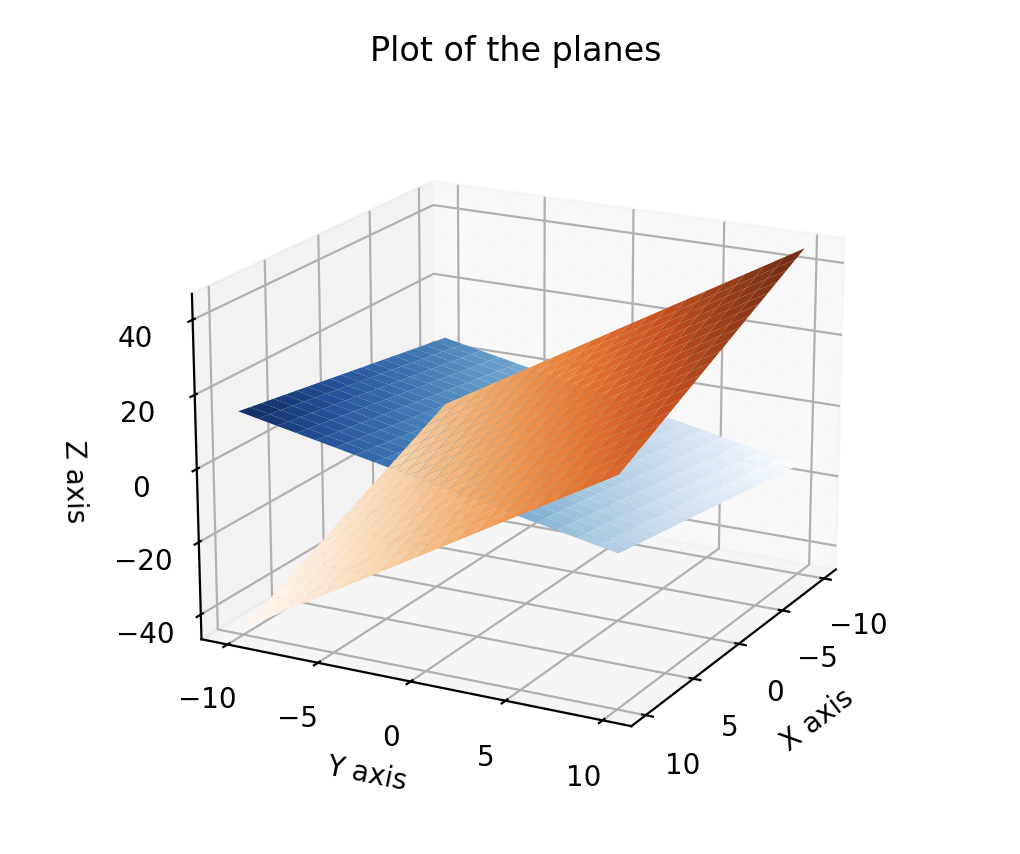
\includegraphics[width=0.7\columnwidth]{Figs/Figure_3.2.png}
    \caption{Plot}
    \label{fig:placeholder}
\end{figure}

\begin{figure}[H]
    \centering
    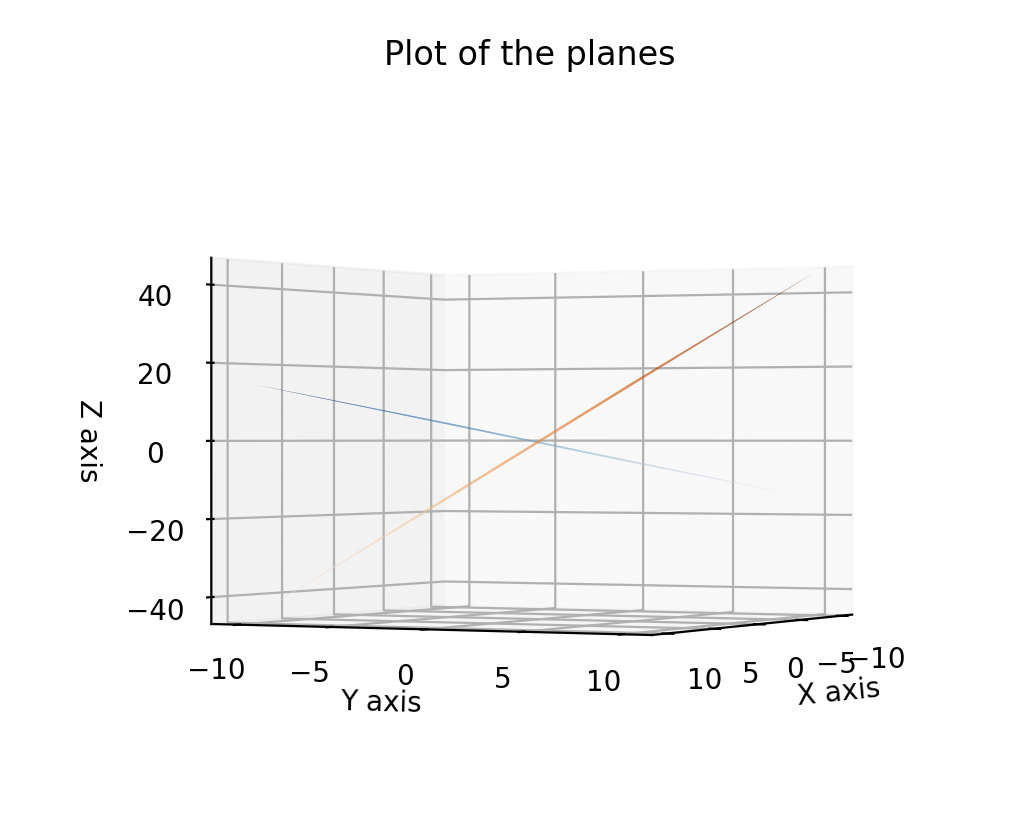
\includegraphics[width=0.9\columnwidth]{Figs/Figure_3.1.png}
    \caption{Plot}
    \label{fig:placeholder}
\end{figure}
\end{document}